% You should title the file with a .tex extension (hw1.tex, for example)
\documentclass[11pt]{article}

\usepackage{algpseudocode}
\usepackage{amsmath}
\usepackage{amssymb}
\usepackage{hyperref}
\usepackage{fancyhdr}
\usepackage{changepage}
\usepackage{amsthm}
\usepackage{graphicx}
\usepackage{listings}
\usepackage{color}
\usepackage{enumitem}
\usepackage{tikz}
\usepackage[normalem]{ulem}
\graphicspath{ {images/} }
\hypersetup{
    colorlinks=true,
    linkcolor=blue,
    filecolor=magenta,      
    urlcolor=cyan,
}
 
\urlstyle{same}

% ------------------------------ Helpful commands ------------------------------

% ---- Question Environment ----
\def\questionskip{\bigskip} % space before each question section
\def\questiontitleskip{\medskip} % space above and below question header
\def\questionleftpadding{0em} % left margin for question section 
\def\questionrightpadding{0em} % right margin for question question 

\newenvironment{question}[2]{ % 2 arguments - question number, question title
  \questionskip
  \hrule
  \questiontitleskip
  \noindent{\bf #1: #2}
  \questiontitleskip
  \hrule \vspace{.10in}
  \begin{adjustwidth}{\questionleftpadding}{\questionrightpadding}
}{
  \end{adjustwidth}
}
% ----------------------------

% ---- Answer Environment ----
\def\answerskip{\smallskip} % space before each answer section
\def\answerleftpadding{1.5em} % left margin for answer section 
\def\answerrightpadding{1.5em} % right margin for answer section 

\newenvironment{answer}
{
  \answerskip
  \color{blue}
  \begin{adjustwidth}{\answerleftpadding}{\answerrightpadding}
  \ttfamily
}{
  \end{adjustwidth}
}
% ----------------------------

% ---- Random Helpful Stuff ----
\newenvironment{letenum}{\begin{enumerate}[label=(\alph*)]}{\end{enumerate}}

\newcommand{\fa}[1]{\forall #1 :}        % Good examples of how to add shortcuts
\newcommand{\ex}[1]{\exists #1 :}       % for text you find youself often typing 
\newcommand{\todo}[1]{\textbf{TODO: #1}\\}
    
\setlength{\parindent}{0pt}
\setlength{\parskip}{5pt plus 1pt}
% ----------------------------

% ------------------------------------------------------------------------------

% ----------------------------- Page Styling & Header --------------------------

\newcommand{\myname}{FirstName LastName}
\newcommand{\myemail}{myemail@university.edu}
\newcommand{\mystudentid}{123456789}
\newcommand{\myclass}{CS-101 }
\newcommand{\myhwnum}{\#1}

\oddsidemargin0cm
\topmargin-2cm            % I recommend adding these three lines to increase the
\textwidth16.5cm           % amount of usable space on the page (and save trees)
\textheight23.5cm

\pagestyle{fancyplain}
\lhead{\fancyplain{}{\textbf{HW\myhwnum}}}        % Note the different brackets!
\rhead{\fancyplain{\myname\\ Student ID: \mystudentid}{\myname\\ \myemail}}

\begin{document}

\thispagestyle{plain}
\begin{flushright}
  \textbf{Worked With:}\\
  Best Friend1\\
  Best Friend2\\
  Best Friend3\\
\end{flushright}

\begin{center}                                      % Center the following lines
  {\Large \myclass Assignment \myhwnum} \\
  \myemail\\
  \today\\
\end{center}
% ------------------------------------------------------------------------------

\begin{question}{Problem 1}{Introduction to the template}
  Hello! This is a simple homework template written in \LaTeX. The goal of the
  of this template is to provide some very light-weight boilerplate to help you
  get started quickly, without getting in your way with overly complex
  styling.\\

  If you are new to Latex, great! It may be a pain at first, but I promise
  after awhile you'll grow to love it. LaTeX has been around forever so while
  that means it has it warts, its mostly good news for us since its usually
  pretty easy to install on most systems (if it isn't already installed by
  default) and there is a great community online, there to help you in your
  time of need! As with most things in life, most of the time if you don't know how
  to do something in LaTeX, a quick Google search will bring you to several
  other people asking the exact same question.\\

  To get started, ShareLaTeX has some great tutorials available on their
  website I'd recommend taking a look at:
  \url{https://www.sharelatex.com/learn/}\\

  Some very basic features that this template provides:
  \begin{itemize}
  \item A number of useful packages imported by default
  \item A question environment
  \item An answer environment (more on this below)
  \item An easy to use makefile
    \begin{itemize}
    \item Run \texttt{make} to build the \textit{homework\_template.tex} file
      (will produce a \textit{homework\_template.pdf} file)
    \item Run \texttt{make example} to build the \textit{example.tex} file (this
      file)
    \item Run \texttt{make clean} to clean up all of the extraneous files
      produced the Latex build proccess
    \end{itemize}
  \end{itemize}
\end{question}


\begin{question}{Problem 2}{Question and Answer Environments}
  Every new question/problem you work on should be wrapped in its own
  ``question'' environment. The question
  \href{https://www.sharelatex.com/learn/Environments}{environment} is a custom
  environment that this template defines and is what is generating all of these
  ``{\bf{Problem \#: Title}}'' headers that you are seeing.\\

  The LaTex code for the question environment, looks like this:\\
  \begin{verbatim} 
\begin{question}{Question Number}{Question Title}
    Your text goes here!!
\end{question}
\end{verbatim}

The template also include an ``answer'' environment you can optionally use. This
is useful when you are including the question text alongside your own work to
help show what is and what is not your work.
\begin{answer}
  The answer environment looks like this and can be nested inside you question
  environment. All it really does is change the font and color of everything
  inside it, while adding padding on both sides. So, don't worry, you can still
  you all of the math you want and use LaTeX as you normally would inside of it.
  \begin{equation}
    \int_a^b f'(x)dx = f(b) -f(a)
  \end{equation}
  and it looks a little something like this:
  \begin{verbatim}
\begin{question}{Question Number}{Question Title}
    You can type the question here...
    \begin{answer}
        And put your answer here!
    \end{answer}
\end{question}
\end{verbatim}
  
\end{answer}
\end{question}

\begin{question}{Problem 3}{Miscellaneous stuff from here on out..}
  \todo{Shortcuts}
  \LaTeX \; makes it wasy for you to define you own commands, which can be super
  helpful if you find yourself repeating things quite often. For example, that
  ``todo'' above is a custom command, helpful to leave in a question if you feel
  like it needs more work and you want to remind youself to come back to it
  later.
  \begin{letenum}
    \item The ``letenum'' environment is a helpful shortcut for a list with
      leters insteand of numbers.
    \item Check the top of either of the template \texttt{tex} file for some
      more examples.
     \item I haven't included many and they are more meant as examples to follow when
       adding your own, but if you think you have some good ones, please let me
       know so I can add them!
  \end{letenum}
\end{question}

\begin{question}{Problem 4}{Psuedo Code}
  If you ever find yourself having to write some psuedocode, you can use the
  \href{https://en.wikibooks.org/wiki/LaTeX/Algorithms#Typesetting_using_the_algorithmicx_package}{algorithmicx}
  package and it's \texttt{algorithmic} environment:\\
  \begin{algorithmic}
    \If {$i\geq maxval$}
    \State $i\gets 0$
    \Else
    \If {$i+k\leq maxval$}
    \State $i\gets i+k$
    \EndIf
    \EndIf
  \end{algorithmic}

  \bigskip
    
  If you find yourself having to write some not-so psuedocode, you can use the
  \href{https://en.wikibooks.org/wiki/LaTeX/Source_Code_Listings}{listings}
  package for some simple syntax highlighting for a multitude of languages.
  \lstset{language=C,
                basicstyle=\ttfamily,
                keywordstyle=\color{olive}\ttfamily,
                stringstyle=\color{red}\ttfamily,
                commentstyle=\color{blue}\ttfamily,
                morecomment=[l][\color{violet}]{\#}
               } 
\begin{lstlisting}[frame=single]
#include <stdio.h>
#define N 10
/* Block
 * comment */

int main()
{
    int i;

    // Line comment.
    puts("Hello world!");
    
    for (i = 0; i < N; i++)
    {
        puts("LaTeX is also great for programmers!");
    }

    return 0;
}
\end{lstlisting}
You can alternatively use the
\href{https://www.sharelatex.com/learn/Code_Highlighting_with_minted}{minted}
package for better syntax highlighting, but it is a little harder to
set up and has an addition Python package dependency and so has
been omitted from this template.
  
\end{question}

\begin{question}{Problem 5}{Graphs, Graphics, and Tables}
  If you need to draw any sort of graph, DFA, etc., I highly recommend
  \href{http://madebyevan.com/fsm/}{Even Wallace's DFA creator}. You can create
  something graphically and then export it to LaTeX.

 \begin{center}
   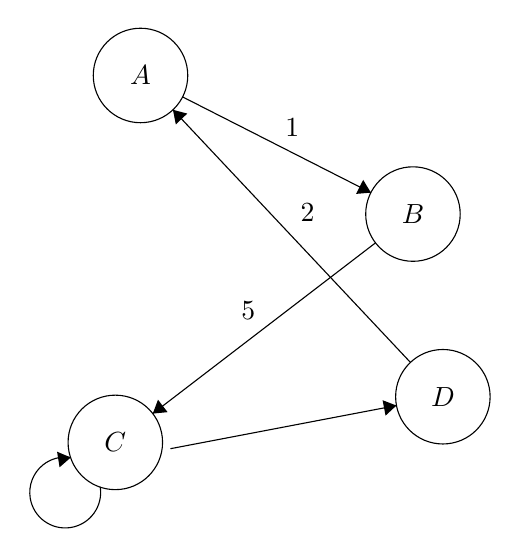
\begin{tikzpicture}[scale=0.2]
     \tikzstyle{every node}+=[inner sep=0pt]
     \draw [black] (19.2,-13.9) circle (3);
     \draw (19.2,-13.9) node {$A$};
     \draw [black] (36.5,-22.7) circle (3);
     \draw (36.5,-22.7) node {$B$};
     \draw [black] (17.6,-37.2) circle (3);
     \draw (17.6,-37.2) node {$C$};
     \draw [black] (38.4,-34.3) circle (3);
     \draw (38.4,-34.3) node {$D$};
     \draw [black] (21.87,-15.26) -- (33.83,-21.34);
     \fill [black] (33.83,-21.34) -- (33.34,-20.53) -- (32.89,-21.42);
     \draw (28.84,-17.8) node [above] {$1$};
     \draw [black] (34.12,-24.53) -- (19.98,-35.37);
     \fill [black] (19.98,-35.37) -- (20.92,-35.28) -- (20.31,-34.49);
     \draw (26.05,-29.45) node [above] {$5$};
     \draw [black] (16.64,-40.03) arc (9:-279:2.25);
     \fill [black] (14.77,-38.16) -- (13.9,-37.79) -- (14.06,-38.78);
     \draw [black] (21.1,-37.6) -- (35.45,-34.86);
     \fill [black] (35.45,-34.86) -- (34.57,-34.52) -- (34.76,-35.5);
     \draw [black] (36.34,-32.12) -- (21.26,-16.08);
     \fill [black] (21.26,-16.08) -- (21.44,-17.01) -- (22.17,-16.32);
     \draw (29.33,-22.63) node [right] {$2$};
   \end{tikzpicture}
 \end{center}

 If you want to include a picture inside your LaTeX homework you can put your
 image in the ''images`` folder and use the \texttt{includegraphics} command.\\
 \begin{center}
   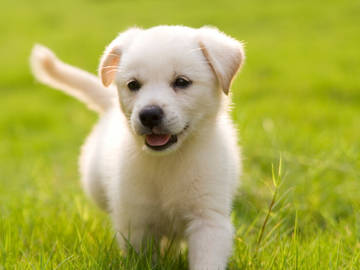
\includegraphics[scale=1.5]{puppy.jpg}
 \end{center}

 You can use the \texttt{tabular} environment for tables. The ampersand ({\bf
   \&}) is used to specify one cell from another and is the common operator for
 most alignment operations in LaTeX.\\

 \medskip
 
 \begin{tabular}{ c | c | c | c | c | c | c  }
   & A & B & C & D & E & F \\
   \hline
   One & 0 & 0 & 0 & 0 & 0 & 0 \\
   Two & 0 & 0 & 0 & 0 & 0 & 0 \\
   Three & 0 & 0 & 0 & 0 & 0 & 0 \\
   Four & 0 & 0 & 0 & 0 & 0 & 0 \\
 \end{tabular}

\end{question}

\begin{question}{Problem 6}{Acknowledgements}
  As with most \LaTeX \; documents, this template \sout{was inspired by}
  shamelessly stolen from a multitude of other \LaTeX \; templates and forum
  comments. I never kept any sort of running list, so I can only thank the
  fantastic online \LaTeX\; community.
\end{question}

\end{document}
